\subsection {Impact on flow completion time}

While stability and fairness are important performance metrics for any
congestion control protocol, the end users often care about flow completion
times, especially for short flows~\cite{rcp}. The fact that TIMELY cannot
maintain a stable queue length has a detrimental impact on flow completion
times, especially at higher percentiles. We illustrate this with a simple
simulation, using the classic dumbbell topology shown in
Figure~\ref{fig:fct_topo}. The topology consists of 20 nodes -- 10 senders and
10 receivers. All traffic flows across the bottleneck link between the two
switches, SW1 and SW2. All links are 10Gbps with 1$\mu$s latency.

The traffic consists  of long and short-lived flows, between pairs of randomly
selected sender and receiver nodes. The flow size distribution is derived from
the traffic distribution reported in~\cite{dctcp}. The interarrival time of
flows is picked from am exponential distribution. The load on the bottleneck
link is varied by changing the mean of the distribution. This traffic generation
model was also used in several recent studies, including pFabric~\cite{pfabric}
and ProjecToR~\cite{projector}. 

Both DCQCN and TIMELY used the default parameter settings recommended
in~\cite{dcqcn} and ~\cite{timely}, respectively. 

The metric of interest is the flow completion time of small flows. Following pFabric~\cite{pfabric}, we define small flows as flows that send fewer than 100KB. Results with other other
thresholds are similar.

Figure~\ref{fig:fct_results} shows the median and 90th percentile of FCT and
DCQCN, TIMELY original and TIMELY (fixed) as the load is varied. TIMELY (fixed) is our modification to TIMELY's protocol to ensure a unique fixed point~\S\ref{sec:timely_fixed}. The X axis shows relative load: load factor of 1 corresponds to an average of 8Gbps of traffic on the bottleneck link. The scaling is linear. We see that at higher loads, FCT for both TIMELY and TIMELY (fixed) is high, and highly variable. The reason is illustrated in detail in Figure~\ref{fig:fct_cdf}, which shows the CDF of the flow completion time for
load factor of 0.8. The reason for TIMELY's poor performance is evident from
Figure~\ref{fig:fct_queue}, which shows the queue length at the link between
SW1 and SW2 for a load factor of 0.8, which shows that queue length under TIMELY
can be high, and highly variable. Note that TIMELY (fixed) is operating in between the original TIMELY protocol and DCQCN. This is because our fix is ensuring a unique fixed point without changing the dynamics of TIMELY's queue build up. 

\begin{figure}[t]
\center
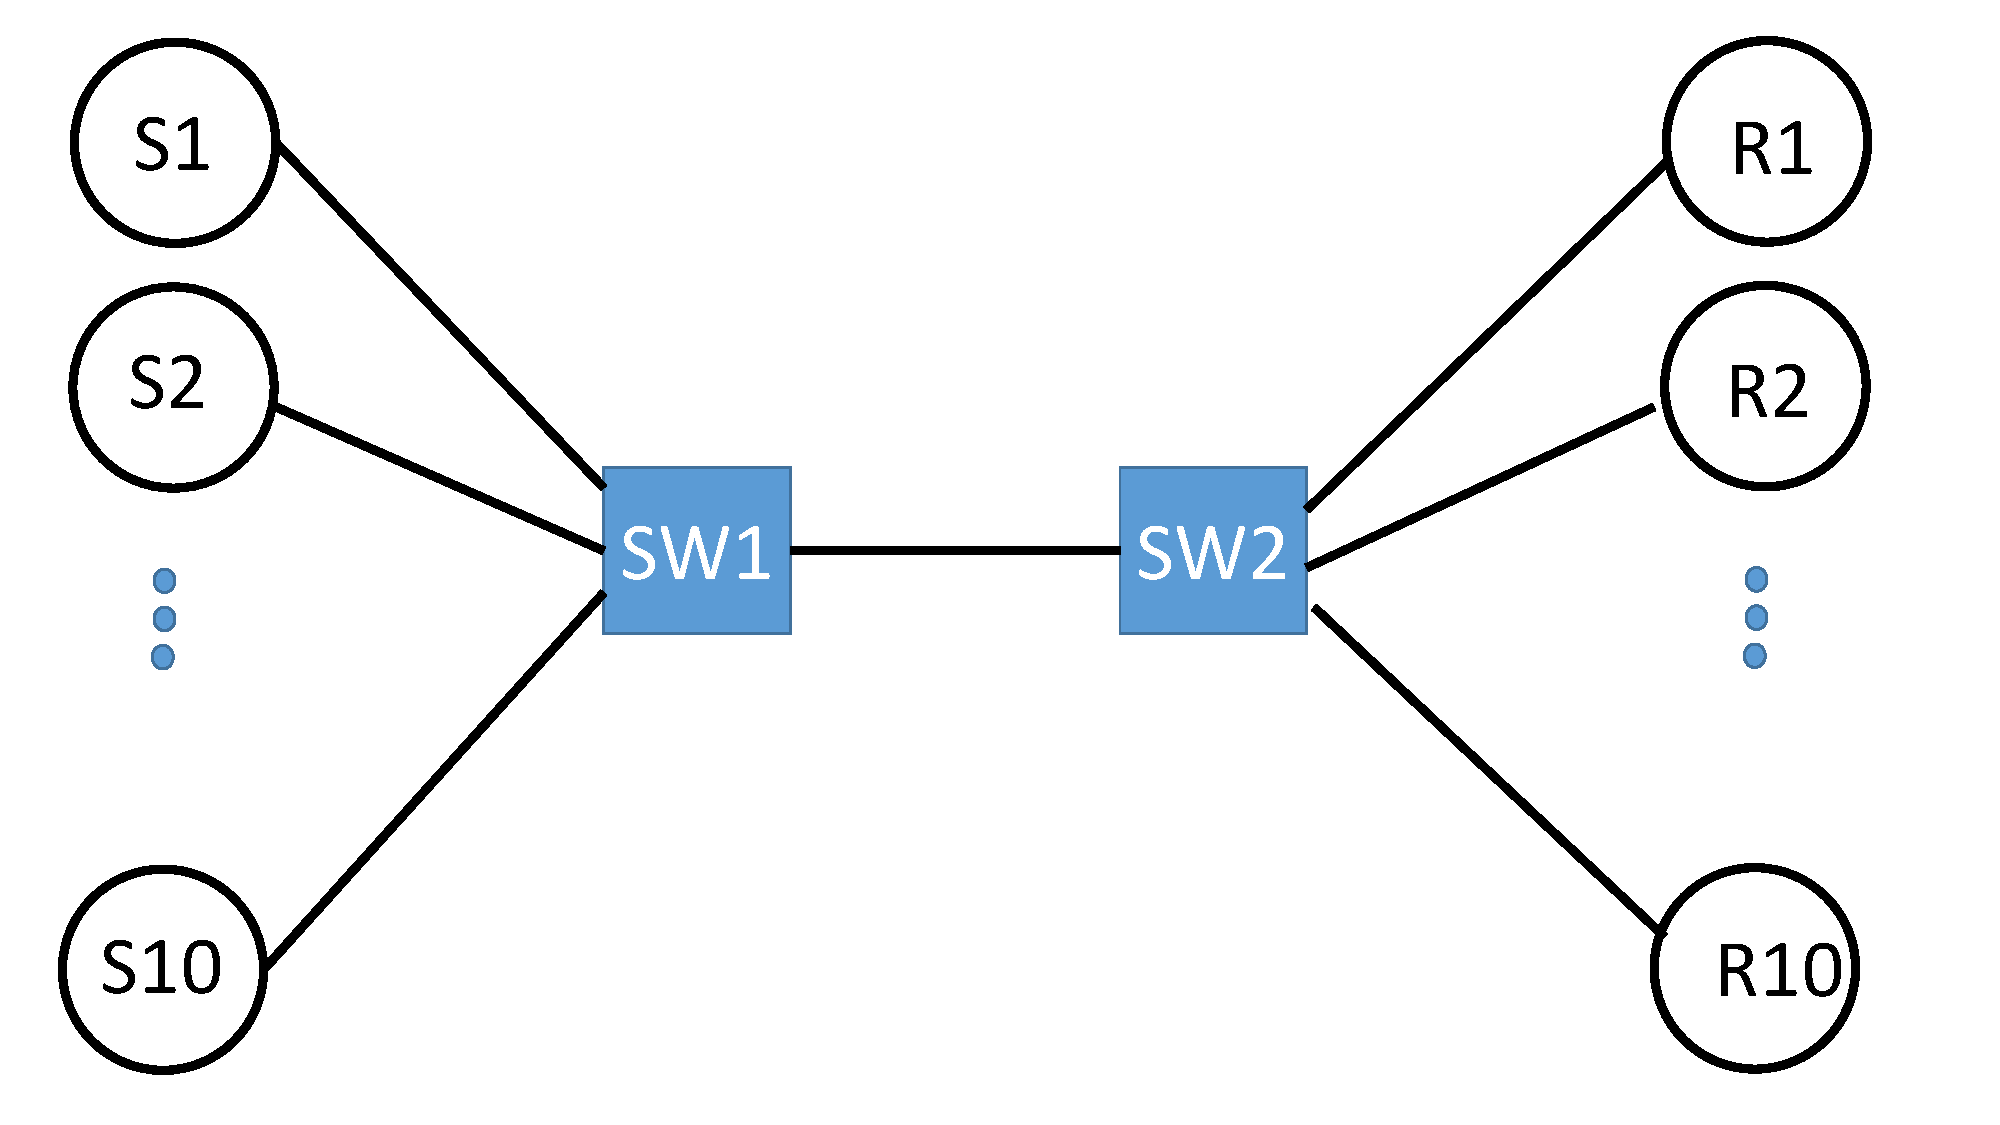
\includegraphics[width=0.3\textwidth]{figures/dumbbell.pdf}
\caption{The dumbbell toplogy. All links are 10Gbps with 1$\mu$s latency.}
\label{fig:fct_topo}
\end{figure}

\begin{figure}[t]
\center
\subfigure []{ 
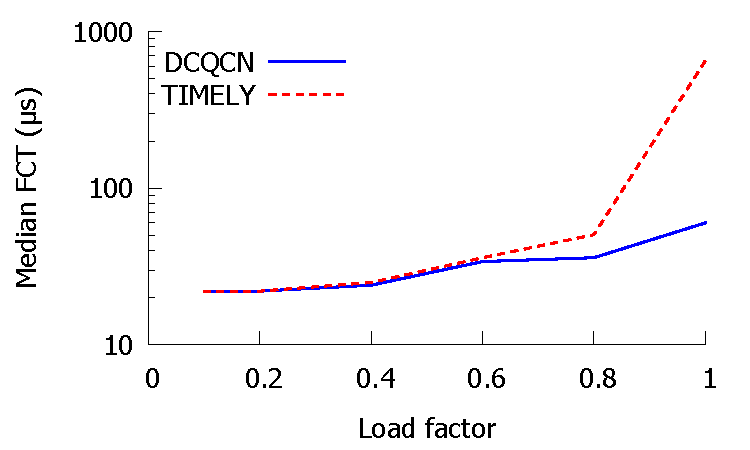
\includegraphics[width=0.3\textwidth]{figures/fct_median.pdf}
\label{fig:fct_median}
}
\subfigure []{ 
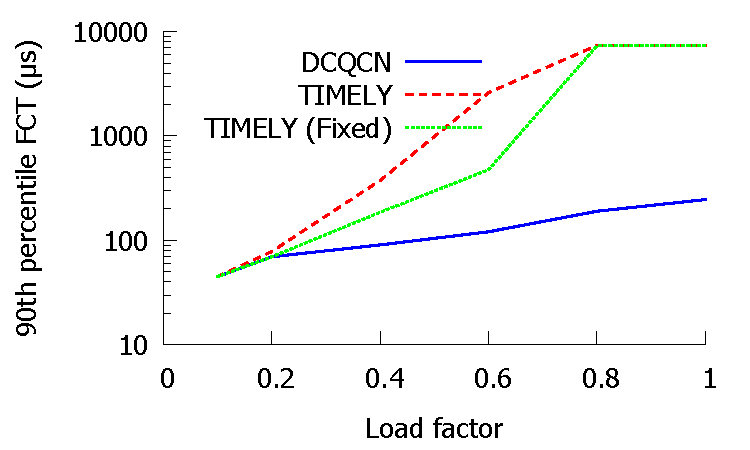
\includegraphics[width=0.3\textwidth]{figures/fct_90.pdf}
\label{fig:fct_90}
}
\caption{Median and 90th percentile of FCT of small flows. Note log scale on Y axis.}
\label{fig:fct_results}
\end{figure}

\begin{figure}[t]
\center
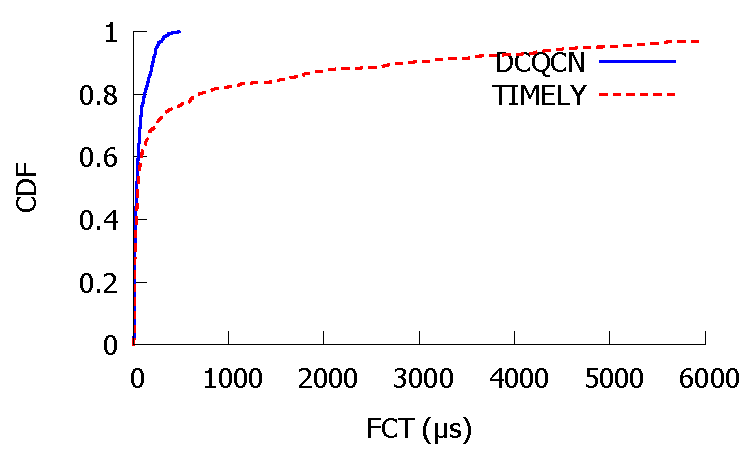
\includegraphics[width=0.3\textwidth]{figures/fct_cdf.pdf}
\caption{CDF of FCT for load=0.8}
\label{fig:fct_cdf}
\end{figure}

\begin{figure}[t]
\center
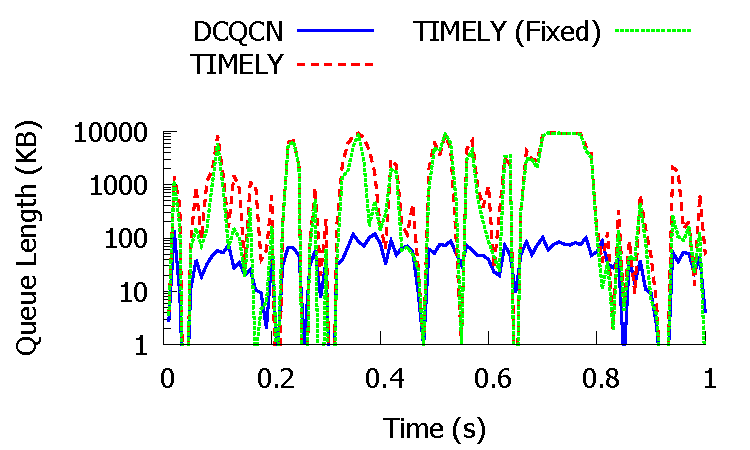
\includegraphics[width=0.3\textwidth]{figures/fct_queue.pdf}
\caption{Bottleneck Queue for load=0.8. Note log scale on Y axis.}
\label{fig:fct_queue}
\end{figure}

We note that in all cases, the link utilization is roughly the same for DCQCN
and TIMELY, indicating that the long flows performed similarly with both
schemes.
